% A skeleton file for producing Computer Engineering reports
% https://kgcoe-git.rit.edu/jgm6496/KGCOEReport_template

\documentclass[CMPE]{../KGCOEReport}

% The following should be changed to represent your personal information
\newcommand{\classCode}{CMPE 260}  % 4 char code with number
\newcommand{\name}{Andrei Tumbar}
\newcommand{\LabSectionNum}{1}
\newcommand{\LabInstructor}{Moskal}    % The slash is to tell LaTeX that the period is between words
% not sentences so it spaces correctly. It won't appear in the
% final pdf
\newcommand{\TAs}{Jacob Meyerson\\Dennis Lam}
\newcommand{\LectureSectionNum}{1}
\newcommand{\LectureInstructor}{Cliver}
\newcommand{\exerciseNumber}{4}
\newcommand{\exerciseDescription}{Execute Stage}
\newcommand{\dateDone}{March 16th}
\newcommand{\dateSubmitted}{March 30th}

\usepackage{tikz}
\usepackage{circuitikz}
\usetikzlibrary{calc}
\usetikzlibrary{circuits.logic.IEC,calc}
\usepackage{multirow}
\usepackage{float}
\usepackage{lmodern}
\usepackage{siunitx}
\usepackage{subcaption}
\usepackage{graphicx}
\usepackage[usestackEOL]{stackengine}
\usepackage{scalerel}
\usepackage[T1]{fontenc}
\usepackage{amsmath}

\def\lbar#1{\ThisStyle{%
    \setbox0=\hbox{$\SavedStyle#1$}%
    \stackengine{2.2\LMpt}{$\SavedStyle#1$}{\rule{\wd0}{0.1\LMpt}}{O}{c}{F}{F}{S}%
}}

\DeclareFontFamily{U}{mathx}{\hyphenchar\font45}
\DeclareFontShape{U}{mathx}{m}{n}{ <-> mathx10 }{}
\DeclareSymbolFont{mathx}{U}{mathx}{m}{n}
\DeclareFontSubstitution{U}{mathx}{m}{n}
\DeclareMathAccent{\widebar}{\mathalpha}{mathx}{"73}

\makeatletter
\newcommand{\cwidebar}[2][0]{{\mathpalette\@cwidebar{{#1}{#2}}}}
\newcommand{\@cwidebar}[2]{\@cwideb@r{#1}#2}
\newcommand{\@cwideb@r}[3]{%
    \sbox\z@{$\m@th\mkern-#2mu#3\mkern#2mu$}%
    \widebar{\box\z@}%
}
\newcommand\currentcoordinate{\the\tikz@lastxsaved,\the\tikz@lastysaved}
\makeatother

\newcommand\decbin[9]{%
    \par\smallskip
    \makebox[3cm][r]{$#1$\ }\fbox{#2}\,\fbox{#3}\,\fbox{#4}\,\fbox{#5}\,\fbox{#6}\,\fbox{#7}\,\fbox{#8}\,\fbox{#9}\par}


\def\code#1{\texttt{#1}}

\begin{document}
    \maketitle
    \section*{Abstract}

    In this laboratory exercise, execute stage and the full ALU were implemented.
    The ALU was missing two vital operations: \code{MUL} and \code{ADD}. A ripple
    carry adder as well as an unsigned integer multiplier were implmented to 
    complete these tasks. The execute stage was modeled to perform ALU 
    functionality given inputs from the decode stage. This exercise was
    successful as it properly implemented the ALU subsystems as well as the
    execute stage and tested their functionality using test benches.

    \section*{Design Methodology}

    \subsection*{ALU Block diagram}
    
    The ALU in this exercise is an extension of the ALU implemented in the
    first exercise. Here, the \code{ADD}, \code{SUB}, and \code{MUL} operations
    are implemented. A 4-select mux will choose between the 9 different
    operations made available by the ALU.
    \\
    The \code{ADD} and \code{SUB} were implemented with the same hardware.
    \code{SUB} simply passed a subtraction operation to the ripple-carry
    adder implementation. The ripple-carry adder is a series of full adders
    where the carry-out from the previous full adder will feed into the
    carry-in of the next full adder. When subtraction was performed, a \code{1}
    was passed to the first full adder and all of the bits of the second operand
    were flipped to get the two's complement form of the number.
    \\
    To implement the \code{MUL} operation, partial products placed into a
    table of bits. Each row would shift over product by one bit.
    Using this table, a product was calculated by summing up all of the rows
    using the ripple carry adder construct. Once added, the output would be
    the product. Inputs into the \code{MUL} circuit were half the size in bits
    that their output so that the output could not overflow.
    \\\\
    A diagram was created to illustrate the functionality of the full ALU.
    
    \begin{figure}[h!]
        \centering
        %! suppress = Ellipsis
        \begin{circuitikz}[american, ]

            \tikzset{mux16/.style={muxdemux,muxdemux def={Lh=16, NL=16, Rh=14, NB=1, w=3, square pins=0}}}
            \tikzset{aluop/.style={dipchip, num pins=4, hide numbers, no topmark, external pins width=0}}

            % Define the inputs
            \draw (-2.5,1) coordinate(A);
            \draw (-2.5,.5) coordinate(B);
            \draw (A) to[multiwire] ++(-0.5,0) node [anchor=east]{A};
            \draw (B) to[multiwire=N] ++(-0.5,0) node [anchor=east]{B};

            % Generate each of the ALU operations are a dipchip
            \def\Ops{
                % Right side
                ADD/0/6,
                MUL/0/4.5,
                OR/0/3,
                AND/0/1.5,
                XOR/0/0,
                SLL/0/-1.5,
                SRL/0/-3,
                SRA/0/-4.5};

            \def\OpPinLength{0.2};
            \def\OpPins{
                % output pin on the right
                out/4/1/left,
                % input pins on the left
                a/1/-1/right,
                b/2/-1/right};

            \foreach \name/\x/\y in \Ops {
                \node [aluop](\name) at (\x,\y) {\name};

                % Generate the input and output pins
                \foreach \subname/\pin/\direction/\labelside in \OpPins {
                    \draw (\name.bpin \pin) -- ++(\OpPinLength*\direction,0) coordinate(\name_\subname);
                    \node [\labelside, font=\tiny] at (\name.bpin \pin) {\subname};
                }
            }

            % Draw the 16 select mux (4 input mux)
            \node [mux16, anchor=lpin 8](ALU) at (4,0){MUX};

            % Label the left pins on the mux in their decimal values
            \foreach \i [evaluate=\i as \pin using int(\i+1)] in {0,...,15} {
                \node [right, font=\tiny] at (ALU.blpin \pin) {\i};
            }

            % Label the select on the mux
            \node [above, font=\tiny] at (ALU.bbpin 1) {op};

            % 4 tuple (CHIP_NAME, BINARY_OPERATOR, MUX_PIN, OFFSET)
            \def\aluinputs{
                ADD/0100 0101/4/0,
                ADD//5/0,
                MUL/0110/6/0,
                 OR/1000/8/0,
                AND/1010/10/0,
                XOR/1011/11/0,
                SLL/1100/12/0,
                SRL/1101/13/0,
                SRA/1110/14/-3};

            \def\ALUpinspace{-0.2} % spacing between output lins
            \def\ALUpinoffset{-0.3} % offset from the ALU lpin

            \def\OpAoffset{-0.2}
            \def\OpBoffset{-0.6}

            % Pins that are not bound to an operation
            \def\undefinedpins{0,1,2,3,7,9,15}

            % Draw connections from the ALU mux pin to the operators output
            % Also add a label for the binary equivalent value
            \foreach \name/\binlabel/\pin/\spacescale [count=\xi, evaluate=\pin as \pinreal using int(\pin+1)] in \aluinputs {
                \draw (ALU.lpin \pinreal) -- ++(\spacescale*\ALUpinspace + \xi*\ALUpinspace + \ALUpinoffset,0)
                    to [short, -] (\currentcoordinate |- \name_out) % go to y-coord for output
                    node[label={[shift={(0,0.3)}, font=\footnotesize] left:\binlabel}] {} % label the wire
                    to[short, -] (\name_out); % connect to the x-coord

                % Connect the input pins on each operator
                \draw (\name_a) -- ++(\OpAoffset,0) to [short, *-*] (\currentcoordinate |- A) -- (A);
                \draw (\name_b) -- ++(\OpBoffset,0) to [short, *-*] (\currentcoordinate |- B) -- (B);
            }

            % Create a ground to handle undefined select pins
            \draw (ALU.south west) ++(-0.4, -0.2) node[sground](g){};

            % Connect the undefined pins to ground
            \foreach /\pin [count=\xi, evaluate=\pin as \pinreal using int(\pin+1)] in \undefinedpins {
                \draw (ALU.lpin \pinreal) -- (g |- \currentcoordinate) to [short, *-] (g);
            }

            % Connect the OP signal to the mux select
            \draw (ALU.bpin 1) to[multiwire=4] ++(0,-2) node [anchor=north] (OP){OP};

            % Connect the output 'Y' signal to the mux output
            \draw (ALU.rpin 1) to[multiwire=N] ++(2,0) node[anchor=west] (Y){Y};

			% connect the operation for add
			\draw (ADD.north) -- ++(0,0.2) node[font=\tiny, anchor=south]{OP(0)};

        \end{circuitikz}
        \caption{Layout of the N-bit ALU with nine operations}
        \label{fig:alublock}
    \end{figure}
    
    \pagebreak
    
    Figure \ref{fig:alublock} shows the functionality of the nine operation
    ALU. Notice that there is no explicit \code{SUB} component. The \code{SUB}
    operation is handled by the \code{ADD} operation by also passing a one bit
    op-code to the adder circuit. When the op-code is \code{1}, the operation
    being performed will be subtraction and vis-versa. Using this functionality
    the ALU operand \code{0101} will output the result from the subtraction
    operation while \code{0100} will output the addition operation's result.
    This is done to eliminate any redundant hardware that would be produced
    from creating two separate adders.
    
    \pagebreak
    
    \subsection*{Execute Stage}
	
	The purpose of the execute stage is to consume inputs from the decode
	stage and perform ALU functionality. Many signals from the decode stage
	are unused and are simply output unchanged. These signals are known as
	"passthroughs".
	The execute stage will feed inputs into the ALU and output the ALU result.
	It will also select between the destination registers \code{RtDest}
	and \code{RdDest} given a control signal \code{RegDst}.
	\\\\
	A block diagram was created to illustrate the functionality of the execute
	stage.
	
	\begin{figure}[h!]
        \centering
        %! suppress = Ellipsis
        \begin{circuitikz}[american, ]
        
        \tikzset{selT/.style={muxdemux, muxdemux def={Lh=2, Rh=1, NL=2, NT=1, NB=0, NR=1, w=1}}}
        \tikzset{selB/.style={muxdemux, muxdemux def={Lh=2, Rh=1, NL=2, NT=0, NB=1, NR=1, w=1}}}
       
       % ALU don't output flags
       \tikzset{ALU/.style={muxdemux,
	 		muxdemux def={Lh=5, NL=2, Rh=2, NR=1, NB=0, NT=1, w=2,
			inset w=1, inset Lh=2, inset Rh=0, square pins=1}}}
       	\draw node[ALU](alu1){\rotatebox{90}{\small \ttfamily ALU}}
       		
       		% simply alu lines
       		(alu1.lpin 1) node[anchor=east]{RegSrcA}
       		(alu1.tpin 1) node[anchor=south]{ALUControl}
       		(alu1.rpin 1) node[anchor=west]{ALUResult}
       		
       		
       		% mux to select ALUSrcB
       		(alu1.lpin 2) node[selB, anchor=rpin 1](aluSel){}
       		(aluSel.lpin 1) node[anchor=east]{RegSrcB}
       		(aluSel.lpin 2) node[anchor=east]{SignImm}
       		(aluSel.lpin 2) ++(0,-0.8) node[anchor=east]{ALUSrc}
       			-| (aluSel.bpin 1)
       	;
       	
       	% WriteReg
       	\draw 
       		(alu1) ++(0,-3.5) node[selB](writeRegSel){}
       		(writeRegSel.lpin 1) node[anchor=east]{RtDest}
       		(writeRegSel.lpin 2) node[anchor=east]{RdDest}
       		(writeRegSel.lpin 2) ++(0,-0.8) node[anchor=east]{RegDst}
       			-| (writeRegSel.bpin 1)
       		(writeRegSel.rpin 1) node[anchor=west]{WriteReg}
       		;
       	
       	% Draw the passthroughs
       	\def\passthrough{
                RegWrite/RegWriteOut,
                MemToReg/MemToRegOut,
                MemWrite/MemWriteOut,
                RegSrcB/WriteData
                };
       	
       	\draw (writeRegSel) ++(-2, -1.5) coordinate(passthroughStart);
       	\foreach \inname/\outname [count=\xi] in \passthrough {
       		\draw (passthroughStart) ++(0,-0.6 * \xi)
       			node[anchor=east]{\inname}
       				-- ++(4,0)
       			node[anchor=west]{\outname}
       		;
       	}
        
        \end{circuitikz}
        \caption{Block diagram of the Execute Stage}
        \label{fig:execblock}
    \end{figure}
	
	Figure \ref{fig:execblock} shows the general functionality of the execute
	state. Most of the heavy lifting in this stage is handled by the ALU. This
	diagram will simply select between two different ALU inputs as well between
	two different destination registers to write to. The bottom four signals
	are simply passthrough signals.
	
    \section*{Results \& Analysis}

	\subsection*{ALU}

    To test the ALU and the Execute Stage, a testbench for each one was
    written. The same input combination was passed to the ALU for each
    operation. A separate ALU was instantiated in the test bench to test
    all of the operations in parallel.
    Expected outputs of the ALU were defined for each operation and asserted
    against to verify their outputs.
    A table of the inputs and expected outputs is shown.
    
    \begin{table}[H]
        \renewcommand{\arraystretch}{1.2}
        \setlength{\tabcolsep}{12pt}
        \caption{Expected outputs of integer operations}
        \begin{center}
            \begin{tabular}{|c|c||c|c|c|}
                \hline
A & B & \code{ADD} & \code{SUB} & \code{MUL}\\\hline

%      A           B         ADD           SUB          MUL
\code{0xA} & \code{0x2} & \code{0xC} & \code{0x8} & \code{0x14}
\\\hline

%      A               B              ADD                 SUB              MUL
\code{0xABCDEF} & \code{0x4} & \code{0xABCDEF16} & \code{0xABCDEF0E} & \code{0x0003BC48}
\\\hline

%      A               B              ADD                 SUB              MUL
\code{0xABCDEF} & \code{0x8} & \code{0xABCDEF1A} & \code{0xABCDEF0A} & \code{0x00077890}
\\\hline

%      A           B            ADD          SUB           MUL
\code{0xAB} & \code{0x7} & \code{0xB2} & \code{0xA4} & \code{0x4AD}
\\\hline
            
            
            \end{tabular}
        \end{center}
        \label{tab:asm}
    \end{table}
    
    \begin{table}[H]
        \renewcommand{\arraystretch}{1.2}
        \setlength{\tabcolsep}{12pt}
        \caption{Expected outputs of logical operations}
        \begin{center}
            \begin{tabular}{|c|c||c|c|c|}
                \hline
A & B & \code{OR} & \code{AND} & \code{XOR}\\\hline

  	%      A           B         OR            AND         XOR
	\code{0xA} & \code{0x2} & \code{0xA} & \code{0x2} & \code{0x8}\\\hline

	%      A               B              OR            AND              XOR
	\code{0xABCDEF} & \code{0x4} & \code{0xABCDEF16} & \code{0x0} & \code{0xABCDEF16} 
	\\\hline

  	%      A               B             OR                 AND            XOR
	\code{0xABCDEF} & \code{0x8} & \code{0xABCDEF1A} & \code{0x0} & \code{0xABCDEF1A}
	\\\hline

  	%      A          B             OR           AND         XOR
	\code{0xAB} & \code{0x7} & \code{0xAF} & \code{0x3} & \code{0xAC}
	\\\hline

            \end{tabular}
        \end{center}
        \label{tab:oax}
    \end{table}
    
    \begin{table}[H]
        \renewcommand{\arraystretch}{1.2}
        \setlength{\tabcolsep}{12pt}
        \caption{Expected outputs of shift operations}
        \begin{center}
            \begin{tabular}{|c|c||c|c|c|}
                \hline
A & B & \code{SLL} & \code{SRA} & \code{SRL}\\\hline

  	%      A           B         SLL            SRA         SRL
	\code{0xA} & \code{0x2} & \code{0x28} & \code{0x2} & \code{0x2}\\\hline

  	%      A               B             SLL                SRA                   SRL
	\code{0xABCDEF} & \code{0x4} & \code{0xBCDEF120} & \code{0xFABCDEF1} & \code{0x0ABCDEF1}
	\\\hline

  	%      A               B             SLL                SRA                   SRL
	\code{0xABCDEF} & \code{0x8} & \code{0xCDEF1200} & \code{0xFFABCDEF} & \code{0x00ABCDEF}
	\\\hline

  	%      A          B             SLL            SRA         SRL
	\code{0xAB} & \code{0x7} & \code{0x5580} & \code{0x1} & \code{0x1}
	\\\hline

            \end{tabular}
        \end{center}
        \label{tab:sss}
    \end{table}
    
    The ALU test cases are shown in Tables \ref{tab:asm}, \ref{tab:oax}, and \ref{tab:sss}.
    All expected outputs are checked for each ALU operations and testcases and will trip
    an assertion failure in the testbench if they are to fail.
    A waveform was generated using this input data.
    
    \begin{figure}[h!]
        \centering
        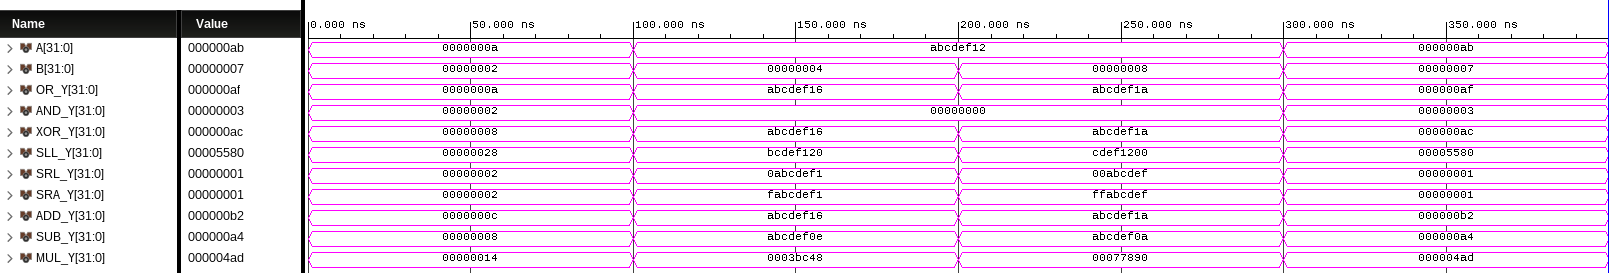
\includegraphics[width=\textwidth]{img/alu_full_behav}
        \caption{Full ALU behavioural waveform}
        \label{fig:alu_behav}
    \end{figure}
    
    \pagebreak
    
    Figure \ref{fig:alu_behav} shows the same 4 input cases for the each operations
    and the expected outputs in the tables above. The ALU is correctly implemented as there
    are no discrepencies between the expected outputs and the real outputs.
    When a working behavioural waveform was generated, a post implementation waveform was
    also generated to show the ALU implementation with timing taken into account.
    
    \begin{figure}[h!]
        \centering
        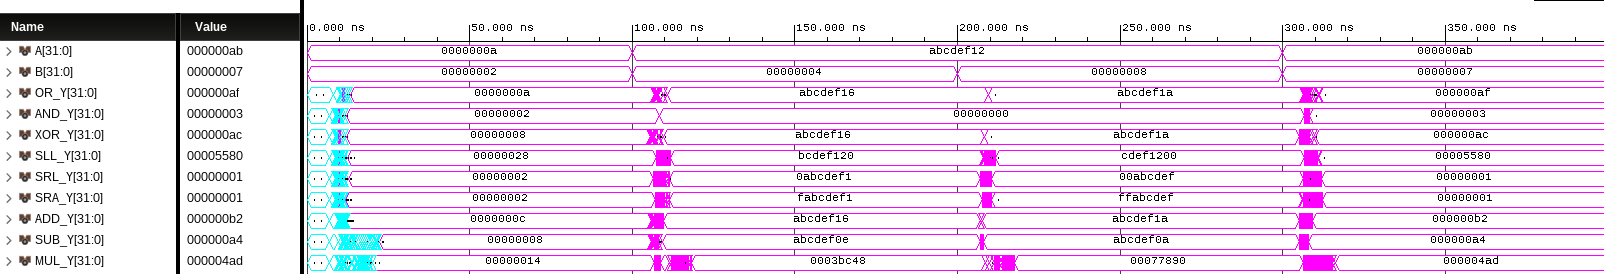
\includegraphics[width=\textwidth]{img/alu_full_impl}
        \caption{Full ALU post-implementation timing waveform}
        \label{fig:alu_impl}
    \end{figure}
    
    Figure \ref{fig:alu_impl} shows the timing and delays of each operation given four
    sets of inputs. It is important to note here that the multiplication circuit has a
    significant delay because the circuit is made up of a chain of ripple-carry adders
    which in turn are a chain of full adders. This complexity will cause a large delay
    in calculating multiplication outputs.

    \subsection*{Execute Stage}

	To test the execute stage, one simply needs to test a small
	subset of the operations of the ALU as well as the execute stage's
	select signals.
	A table is shown to illustrate the nature of the execute stage's 
	test bench.
	
	\begin{table}[H]
        \renewcommand{\arraystretch}{1.2}
        \setlength{\tabcolsep}{12pt}
        \caption{Inputs and expected outputs of Execute Stage}
        \begin{center}
            \begin{tabular}{|c|c|c|c|c||c|}
                \hline
RegSrcA & RegSrcB & SignImm & ALUSrc & ALUOp & ALUResult\\\hline

  	%      A           B      SignImm       ALUSrc     Op   ALUResult
	\code{0x0} & \code{0x3} & \code{--} & \code{0} & \code{ADD} & \code{0x3}
	\\\hline

  	%      A           B      SignImm       ALUSrc     Op   ALUResult
	\code{0x2} & \code{--} & \code{0xffffffff} & \code{1} & \code{ADD} & \code{0x1}
	\\\hline

  	%      A           B      SignImm       ALUSrc     Op   ALUResult
	\code{0xFF} & \code{--} & \code{0x8} & \code{1} & \code{SLL} & \code{0xFF00}
	\\\hline

  	%      A           B      SignImm       ALUSrc     Op   ALUResult
	\code{0xABCD} & \code{0xFFFF} & \code{--} & \code{0} & \code{MUL} & \code{0xabcc5433}
	\\\hline

            \end{tabular}
        \end{center}
        \label{tab:exec}
    \end{table}
	
	Table \ref{tab:exec} shows the inputs and expected output of the execute
	stage. All of the passthrough output signals shown in Figure
	\ref{fig:execblock} are automatically tested by passing an alternating
	signals to the inputs and verifying the outputs are the same. Notice how
	SignImm and RegSrcB are marked with \code{--} or dont-care when the
	ALUSrc is not selecting them as an input to the ALU. This test only runs
	a subset of the valid ALU operations because its purpose is to test only the
	Execute stage.
	Waveforms were generated for the testcases outlines in Table \ref{tab:exec}.
	
	\begin{figure}[h!]
        \centering
        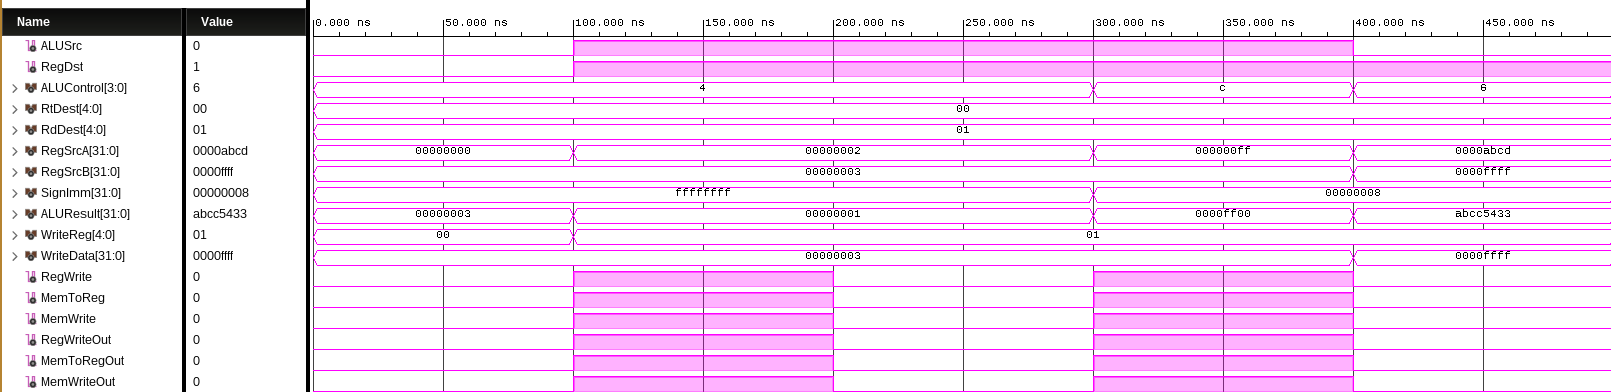
\includegraphics[width=\textwidth]{img/exec_2_behav}
        \caption{Full Execute Stage behavioural waveform}
        \label{fig:exec_behav}
    \end{figure}
   	
   	A post-implementation timing simulation was also run for the
   	execute stage to show the delays associated with this component.

	\begin{figure}[h!]
        \centering
        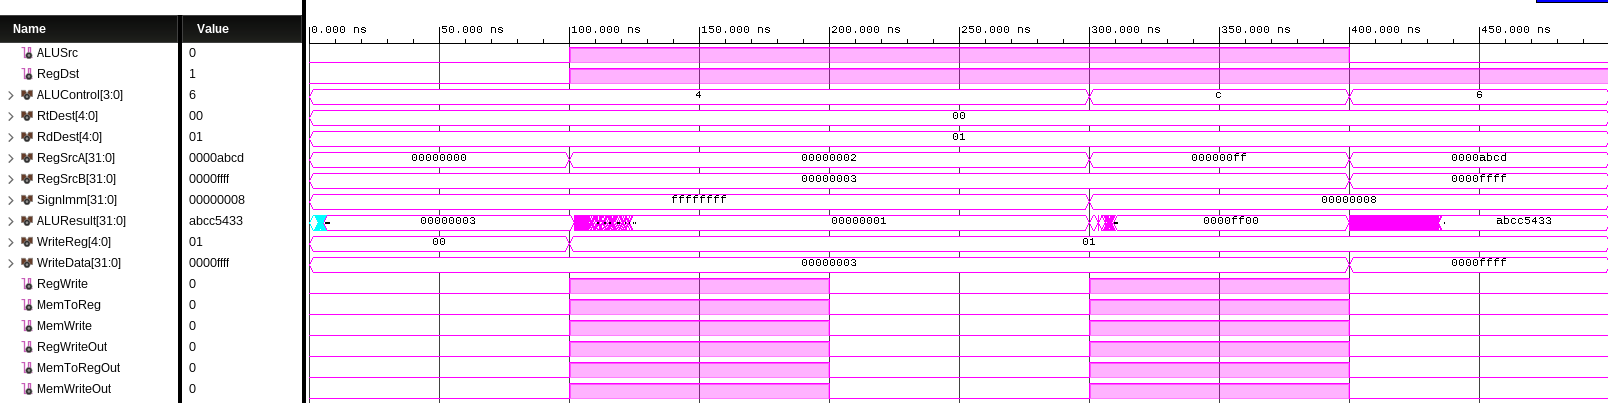
\includegraphics[width=\textwidth]{img/exec_2_impl}
        \caption{Full Execute Stage post-implementation timing waveform}
        \label{fig:exec_impl}
    \end{figure}
    
    The delays shown in Figure \ref{fig:exec_impl} are slightly
    longer than the ones shown in Figure \ref{fig:exec_behav}
    because there is extra logic to select between the ALU inputs.
    Because of this long delay seen in the execute stage, the clock
    period may not be shorter than about 30ns and the execute stage
    should be placed in its own clock cycle in the pipeline. This is because
    any shorter clock period will result in passing an unstable value through
    the pipeline for \code{MUL} operations.
    

    \section*{Conclusion}
    This laboratory exercise the complete ALU along with the MIPS execute
    stage were implemented. To finish the ALU from exercise 1, a ripple carry
    adder and an unsigned integer multipier circuit were written. The execute
    stage provided some logic to select inputs into the ALU as well as passthrough
    signals given from the decode stage. This exercise was successful as it
    properly implementation the ALU and Execute stage with a proper corpus of
    tests written for each component.

    \pagebreak

    \section*{Demo results}
    
    \subsection*{Part1}
    \begin{figure}[h!]
        \centering
        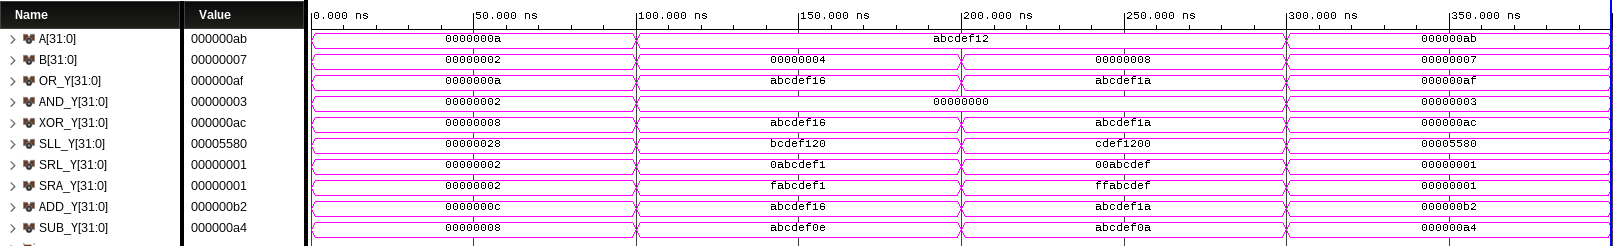
\includegraphics[width=\textwidth]{img/alu_behav}
        \caption{Behavioural simulation of ALU (without MUL)}
        %! suppress = FigureNotReferenced
        \label{fig:demo1}
	\end{figure}
    \begin{figure}[h!]
        \centering
        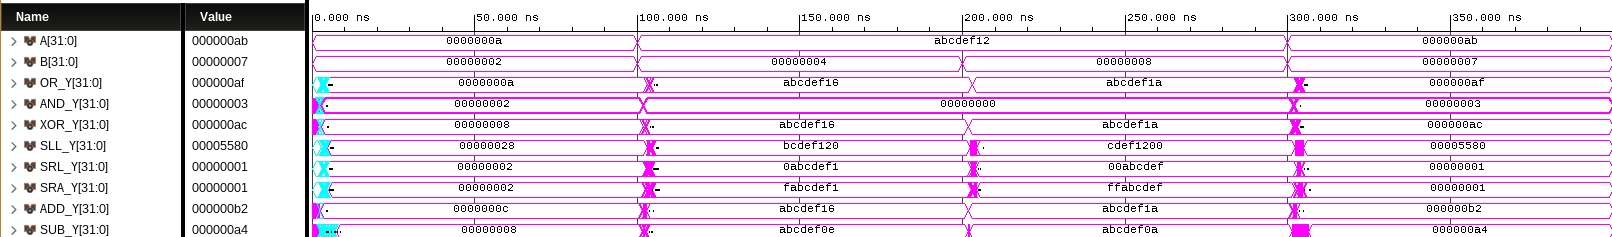
\includegraphics[width=\textwidth]{img/alu_synth}
        \caption{Post-synthesis timing simulation of ALU}
        %! suppress = FigureNotReferenced
        \label{fig:demo1}
	\end{figure}
    \begin{figure}[h!]
        \centering
        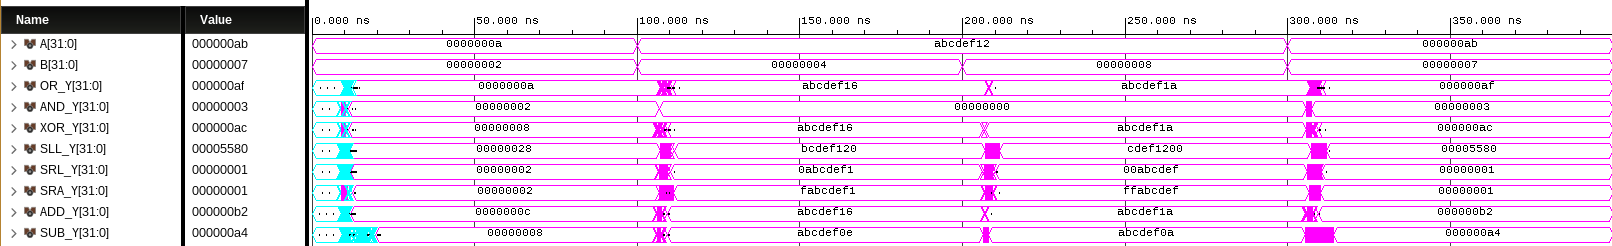
\includegraphics[width=\textwidth]{img/alu_impl}
        \caption{Post-implementation timing simulation of ALU}
        %! suppress = FigureNotReferenced
        \label{fig:demo1}
	\end{figure}
    \begin{figure}[h!]
        \centering
        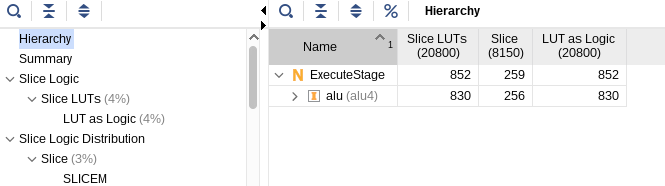
\includegraphics[width=\textwidth]{img/util_report}
        \caption{Utilization report on Baysis 3 board}
        %! suppress = FigureNotReferenced
        \label{fig:demo1}
	\end{figure}
    \begin{figure}[h!]
        \centering
        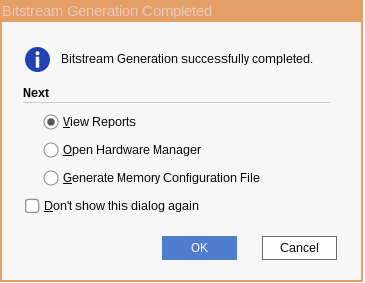
\includegraphics[width=\textwidth/2]{img/bitstream_successful}
        \caption{Bitstream successfully generated for 4-bit ALU}
        %! suppress = FigureNotReferenced
        \label{fig:demo1}
	\end{figure}
    \subsection*{Part2}
	\begin{figure}[h!]
        \centering
        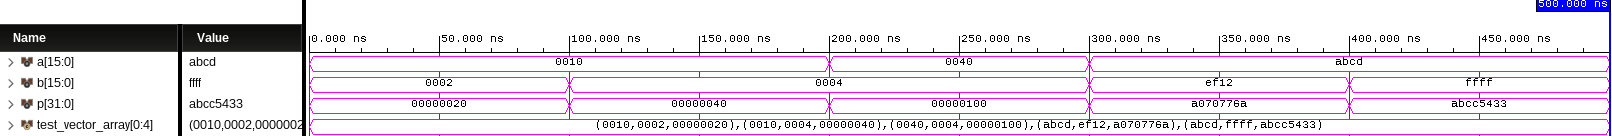
\includegraphics[width=\textwidth]{img/mult_behav}
        \caption{Behavioral simulation of multiply}
        %! suppress = FigureNotReferenced
        \label{fig:demo1}
	\end{figure}
	\begin{figure}[h!]
        \centering
        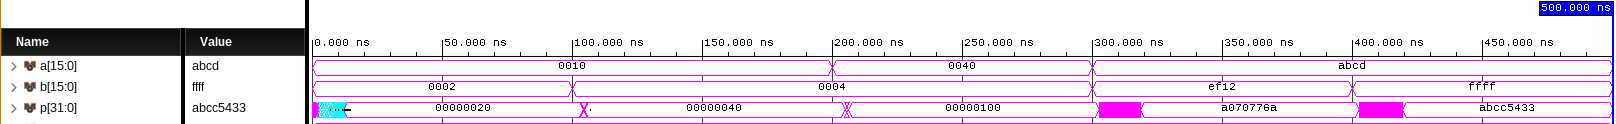
\includegraphics[width=\textwidth]{img/mult_synth}
        \caption{Post-synthesis timing simulation of multiply}
        %! suppress = FigureNotReferenced
        \label{fig:demo1}
	\end{figure}
	\begin{figure}[h!]
        \centering
        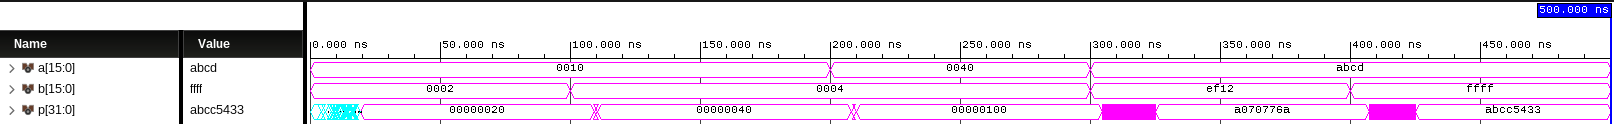
\includegraphics[width=\textwidth]{img/mult_impl}
        \caption{Post-implementation timing simulation of multiply}
        %! suppress = FigureNotReferenced
        \label{fig:demo1}
	\end{figure}
	\begin{figure}[h!]
        \centering
        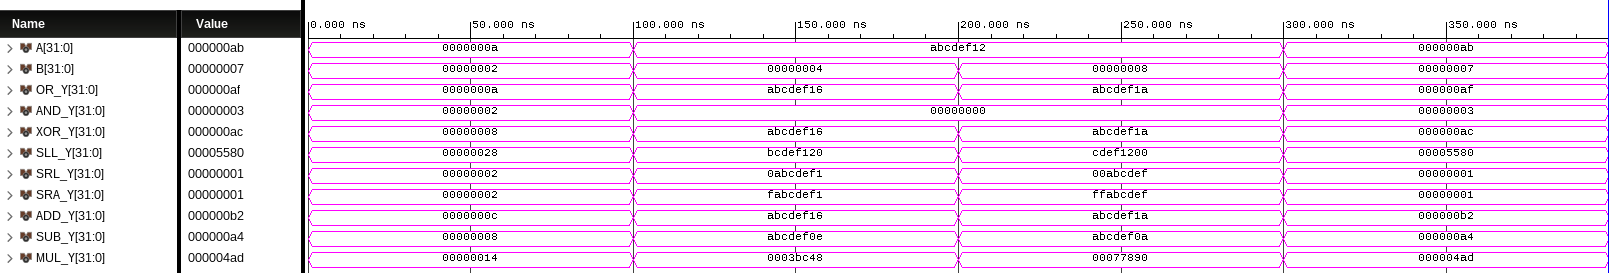
\includegraphics[width=\textwidth]{img/alu_full_behav}
        \caption{Full ALU behavioral simulation}
        %! suppress = FigureNotReferenced
        \label{fig:demo1}
	\end{figure}
	\begin{figure}[h!]
        \centering
        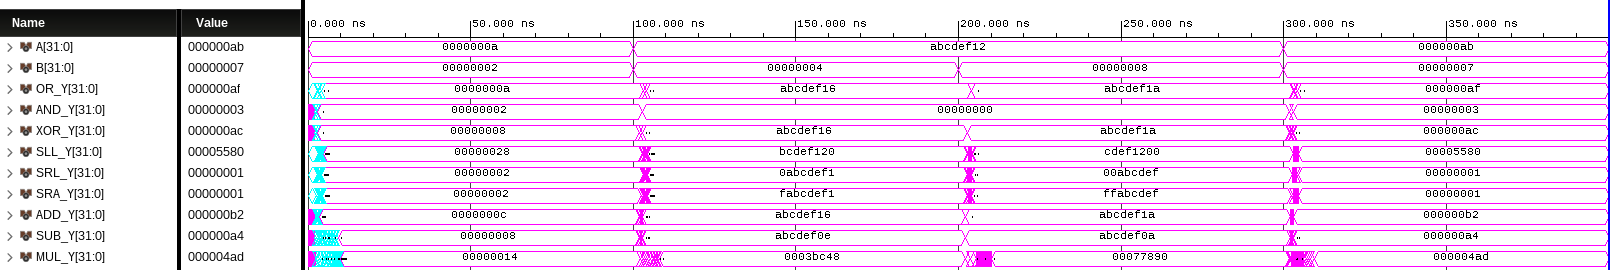
\includegraphics[width=\textwidth]{img/alu_full_synth}
        \caption{Post-synthesis timing simulation of full ALU}
        %! suppress = FigureNotReferenced
        \label{fig:demo1}
	\end{figure}
	\begin{figure}[h!]
        \centering
        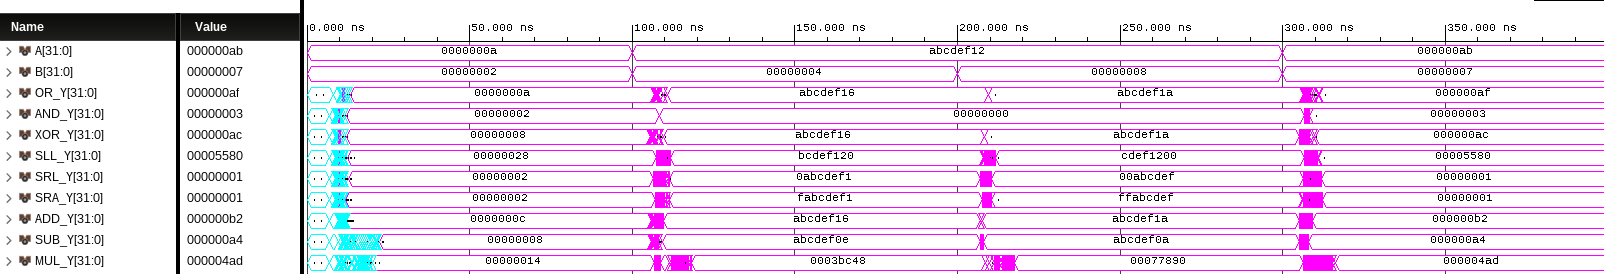
\includegraphics[width=\textwidth]{img/alu_full_impl}
        \caption{Post-implementation timing simulation of full ALU}
        %! suppress = FigureNotReferenced
        \label{fig:demo1}
	\end{figure}
	\begin{figure}[h!]
        \centering
        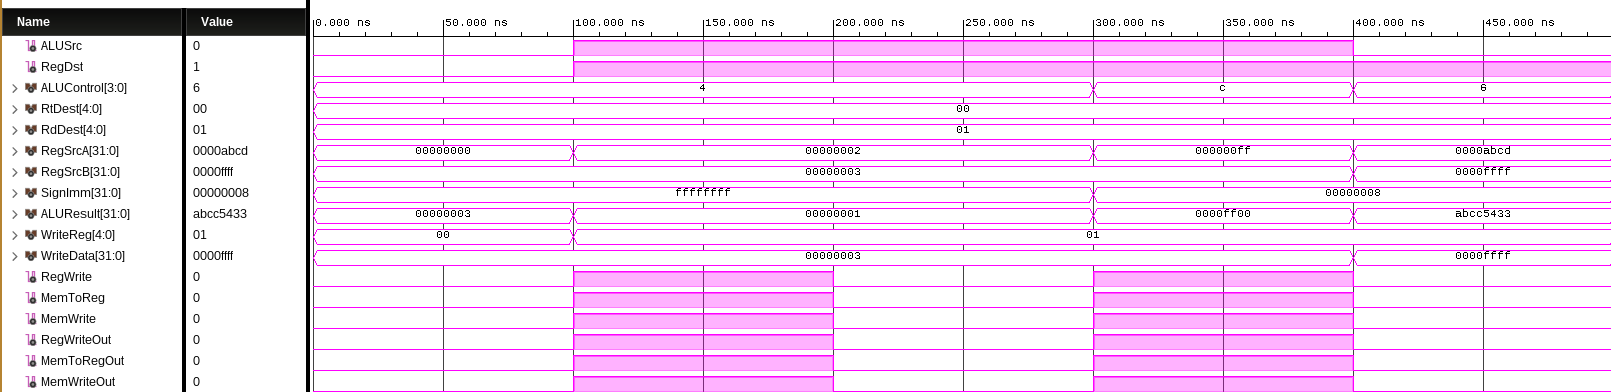
\includegraphics[width=\textwidth]{img/exec_2_behav}
        \caption{Complete Execute Stage behavioral simulation}
        %! suppress = FigureNotReferenced
        \label{fig:demo1}
	\end{figure}
	\begin{figure}[h!]
        \centering
        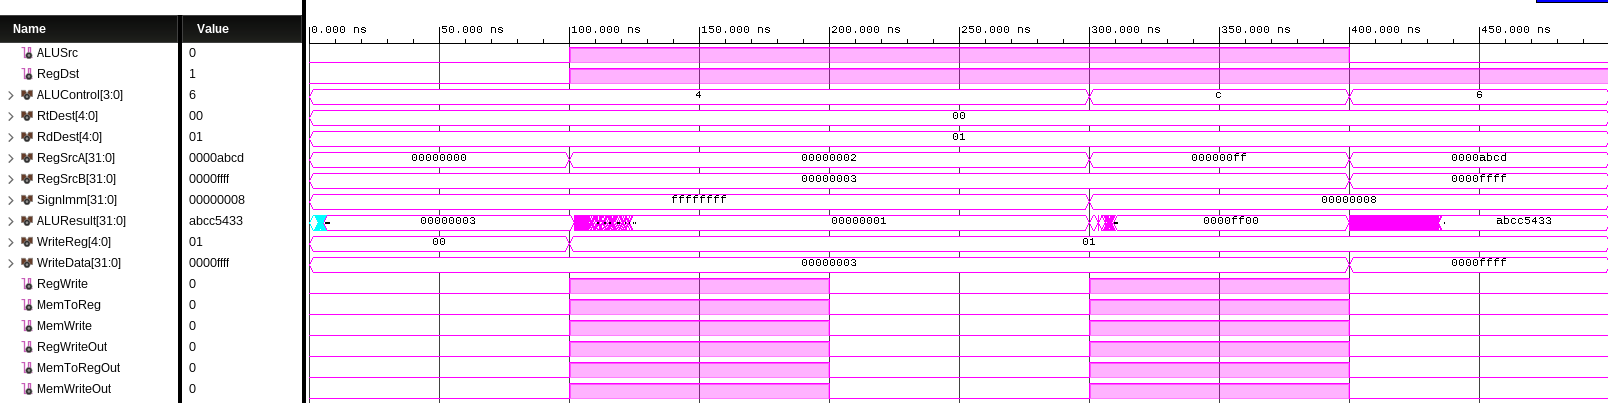
\includegraphics[width=\textwidth]{img/exec_2_impl}
        \caption{Complete Execute Stage post-implementation timing simulation}
        %! suppress = FigureNotReferenced
        \label{fig:demo1}
	\end{figure}

\end{document}